\documentclass{beamer}
\usetheme{Luebeck}
\usecolortheme{seahorse}
\usefonttheme{structurebold,serif}
\setbeamertemplate{navigation symbols}{\usebeamerfont{footline}\insertframenumber/\inserttotalframenumber}
\usepackage{luatexja-fontspec}
\setmainfont{STIX Two Text}
\setsansfont{Helvetica}
\setmonofont{Inconsolata}
\setmainjfont{YuKyo_Yoko-Medium}[BoldFont=YuKyo_Yoko-Bold]
\setsansjfont{YuGo-Medium}[BoldFont=YuGo-Bold]
\usepackage{mathtools}
\usepackage[warnings-off={mathtools-colon,mathtools-overbracket}]{unicode-math}
\unimathsetup{math-style=ISO,bold-style=ISO}
\setmathfont{STIX Two Math}
\mathtoolsset{showonlyrefs=true}
\usepackage{graphicx}
\title{ソリトンとリー代数}
\author{宇佐見 公輔}
\date{2023年2月11日}
\begin{document}
\maketitle

\begin{frame}
    \frametitle{はじめに}

    今年1月に佐藤幹夫先生が亡くなられました。

    \bigskip
    佐藤幹夫先生の業績はいろいろとありますが、個人的にはソリトン理論が印象深いです。

    \bigskip
    今回は、佐藤幹夫先生の理論を中心にソリトン研究の歴史について話します。

    \bigskip
    なお、このあたりの話はすでに専門家による優れた解説文や書籍があります。
    もし興味を持った方がおられたら、それらをぜひご参照ください。
\end{frame}

\begin{frame}
    \frametitle{線形な波・非線形な波}

    波は微分方程式で記述される。

    たとえば、真空中の電磁波は以下の方程式で記述される。
    \begin{equation}
        \frac{∂^2u}{∂t^2}=c^2\frac{∂^2u}{∂x^2}
    \end{equation}

    \bigskip
    線形な波:
    \begin{itemize}
        \item 解と解の和も解になる(重ね合わせの原理)。
        \item 真空中の電磁波などがある。
    \end{itemize}

    \bigskip
    非線形な波:
    \begin{itemize}
        \item 解と解の和が解になるとは限らない。
        \item 水面の波などがある。
    \end{itemize}
\end{frame}

\begin{frame}
    \frametitle{ソリトン}

    非線形な波は通常、波と波が衝突すると形が崩れて元に戻らない。

    \bigskip
    しかし、非線形な孤立波でありながら、衝突しても崩れないものがある。
    これをソリトンと呼ぶ(1965年にザブスキーとクルスカルによって命名された)。

    \bigskip
    ソリトン解を持つ非線形方程式は、たとえばKdV方程式がある。
    ほかにも、KP方程式、非線形シュレディンガー方程式、サイン-ゴルドン方程式、戸田格子、などがある。
\end{frame}

\begin{frame}
    \frametitle{ソリトンの発見}

    1834年、ラッセルが、エジンバラの運河で形を変えない水面波(ソリトン)を観測。
    この孤立波に関する実験をおこなう。

    \bigskip
    1895年、コルテヴェーグとド・フリースが、ラッセルの波に対応する微分方程式(KdV方程式)を提出。
    $1$-ソリトン解を求める。
    \begin{equation}
        \frac{∂u}{∂t}+6u\frac{∂u}{∂x}+\frac{∂^3u}{∂x^3}=0
    \end{equation}

    \bigskip
    ソリトン発見当時は、特定の方程式に対する特殊事情と思われていた。
    また、非線形方程式であるため、研究が困難だった。
\end{frame}

\begin{frame}
    \frametitle{逆散乱法}

    1965年、ザブスキーとクルスカルが、コンピューターによる実験でKdV方程式の$1$-ソリトン解を得る。

    \bigskip
    1967年、ガードナー、グリーン、クルスカル、ミウラが、逆散乱法でKdV方程式の$N$-ソリトン解を求める。

    \bigskip
    逆散乱法の成功を機に、ソリトンの数理的研究が盛んになる。
    この時代にさまざまなソリトン方程式が発見され解かれる。

    \bigskip
    ソリトン方程式は「無限自由度の可積分系」として数学の研究対象となる。
\end{frame}

\begin{frame}
    \frametitle{佐藤理論}

    1970年代、広田が、ソリトン方程式に対する広田の直接法を考案する。
    逆散乱法を使わず、双線形方程式に変換して解く手法。

    \bigskip
    1981年、佐藤幹夫が、KP方程式(ソリトン方程式)の解全体がグラスマン多様体をなすことを示す。

    \bigskip
    これによって、広田の直接法の幾何的・代数的な意味がわかるとともに、ソリトン方程式の可積分性の根源が見えてきた。

    \bigskip
    これを機にさまざまな可積分系の代数的構造の研究が盛んになる。

\end{frame}

\begin{frame}
    \frametitle{ソリトン方程式とアフィンリー代数}

    1970年代、素粒子論の研究で頂点作用素という概念が現れた。

    \bigskip
    1978年、レポウスキー、ウィルソン、カッツ、フレンケルが、頂点作用素がアフィンリー代数の実現と結びつくことを発見する。

    \bigskip
    1981年、伊達、神保、柏原、三輪が、ソリトン方程式の解の変換群のリー代数がアフィンリー代数であることを示す。

    \bigskip
    これによって、ソリトン方程式や可積分系とアフィンリー代数が関連していることが見出された。
    また、ソリトンや可積分系にある対称性が見えてきた。
\end{frame}

\begin{frame}
    \frametitle{その後の展開}

    1970年代〜1980年代は、ソリトンに限らず、物理と数学とで別個に研究されていたさまざまな事柄が結びついていった時代。

    \bigskip
    統計物理の格子模型がアフィンリー代数と関連していることが見出されたのもこのころ。
    格子模型はソリトンとも関連がある。

    \bigskip
    また、リー代数の変形が研究され、量子群が生まれた。
    量子群は数理物理のさまざまなところで関連がある。
\end{frame}

\begin{frame}
    \frametitle{余談(最近個人的におもしろかったこと)}

    Perplexityに何気なくOnsager代数のことを質問したら、以前に僕が関西日曜数学友の会で話した件が返ってきた。

    \begin{center}
        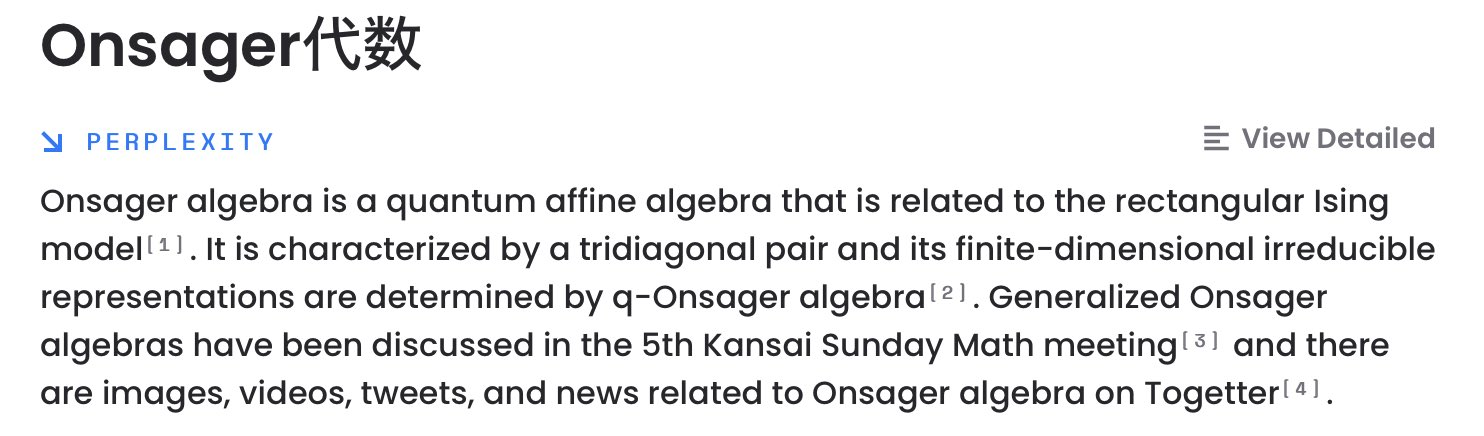
\includegraphics[scale=0.2]{Perplexity.jpeg}
    \end{center}

    チャットAI、日曜数学の情報まで捕捉しているとは。
\end{frame}

\begin{frame}
    \frametitle{参考文献}

    \begin{block}{上野喜三雄、ソリトンがひらく新しい数学、岩波書店、1993}
        理論が生まれた当時の熱気が伝わってくる読みものです。
        今回の話はこの本の内容をベースにしました。
    \end{block}

    \begin{block}{三輪哲二・神保道夫・伊達悦朗、ソリトンの数理、岩波書店、1993}
        理論の内容を詳しく解説した本です。
        もともとは岩波講座応用数学シリーズのなかの1冊で、2007年に単行本化され、2016年には岩波オンデマンド版が出ています。
    \end{block}
\end{frame}

\end{document}
